\section{Solution Design and Implementation}
\label{sec:parallelization}

\subsection{Parallelization With OpenMPI}
To harness the speedups offered by parallel computing, we used the OpenMPI library.
The first step was to choose which part of the program to parallelize.
This has been easy: the recursive part.
the points are divided among the processes, then merged.
It was now time to decide how to communicate amongst processes, and we came up with the scheme of which in \Cref{fig:albero_bell_albero}.
The splitting of the work can be visualized as a tree, in which each node does the same amount of work. The nodes on the left communicate to the nodes on the right.

\begin{figure}[!ht]
    % \resizebox{\columnwidth}{!}{
    %     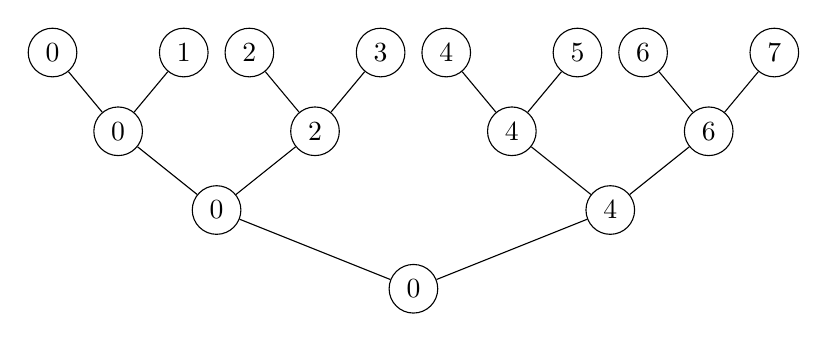
\begin{tikzpicture}[
        grow'=up,
        every node={
                style={
                        draw,align=center
                    }
            },
        level distance=1cm,
        level/.style={sibling distance=5cm/#1}
    ]
    \tikzset  {
        treenode/.style = {circle, draw=black, align=center, minimum size=0.5cm},
    }
    \node [treenode] {0}
    child {
            node [treenode] {0}
            child
                {
                    node [treenode] {0}
                    child {
                            node [treenode] {0}
                        }
                    child {
                            node [treenode] {1}
                        }
                }
            child
                {
                    node [treenode] {2}
                    child {
                            node [treenode] {2}
                        }
                    child {
                            node [treenode] {3}
                        }
                }
        }
    child {
            node [treenode] {4}
            child
                {
                    node [treenode] {4}
                    child {
                            node [treenode] {4}
                        }
                    child {
                            node [treenode] {5}
                        }
                }
            child
                {
                    node [treenode] {6}
                    child {
                            node [treenode] {6}
                        }
                    child {
                            node [treenode] {7}
                        }
                }
        }
    ;
\end{tikzpicture}

    % }
    \centering
    \includesvg{../assets/graphics/tree_merge.svg}
    \caption{Illustration of the process communication scheme with 8 processes.}
    \label{fig:albero_bell_albero}
\end{figure}

It was now time to implement it with OpenMPI. This required several modifications to the code. The first thing was to decide which MPI calls to make.
Process 0 is the one that reads the file initially and then reassembles the final result.
The natural choice at the beginning to distribute the points was a \verb+MPI_Scatterv+. To do this we had to implement two MPI datatypes, \verb+mpi_point_type+ to represent a point and \verb+mpi_pair_of_points_type+
to represent a pair of points.
Then each process receives its points and can work on them. Each process knows how many points to receive since they received the total count of points from 0 with a broadcast.
After the process computed its closest pair, it calculates the bands according to the smallest distance it found and sends them to the receiving process.
This would call for four MPI send operations (left band count, right band count, left band points, right band points). Instead, we optimized this by sending the two lengths simultaneously and then the concatenation of the band points.

\subsection{CI/CD Setup}

Writing code is undoubtedly a core part of the process, yet as the complexity of the projects grow, good software engineering practices become more and more important in helping to keep the growth of the codebase under control.
%As in security, we like to remove things that can fail from the loop, and these are humans. Sorry humans.
In our case, we decided to set up a version control system with git\footnote{\url{https://git-scm.com}} from the get-go, hosting on GitHub. After that, we added Continuous Integration through the use of GitHub Actions and Google Test framework\footnote{\url{https://google.github.io/googletest}}. The CI pipeline is minimal, but effective in preventing regressions: every time a push (or pull request) is made, the code is compiled -with the same compiler, mpicc, that is used on the cluster- and tests are run. Our actual tests perform a small run of the algorithm in order to check if it outputs the expected result.

If everything until now went well, the GitHub Action proceeds in doing a small test run on the cluster. In order to do so, it copies the source code to the cluster, compiles it and submits a job with a medium sized dataset -1M points-, asking for 2 CPUs and 2 nodes, with a time limit of 5 minutes. When the job completes -or fails-, we are notified through a Telegram bot, which also sends us the output files. Each job is created in its own subdirectory, so everything is retained if we need to check back on it later on.
Since we are running on a shared cluster, our scripts also include automatic checks to ensure we are not using more storage than we are allowed to use.

We also produced another pipeline for the automatic execution of the benchmark tests. These are managed by a pipeline that is triggered when we create a new tag in the repository.
The benchmark pipeline executes the same tests as the other pipeline, with the only difference that instead of creating a single job, it sequentially submits to the cluster -one at a time- all the configurations of inputs and job parameters we want to test -namely, number of nodes, number of CPUs, and packing strategy-. The script checks the status of the submitted job every 10 seconds. Once the job is finished, it collects its results and adds them to a new row in a google spreadsheet
\footnote{Link in \Cref{link:spreadsheet}}.
The benchmarking scripts executes everything four times, and notifies us on Telegram as it progresses and when it finishes.
As with the CI, everything in the cluster is neatly organized in its own subdirectory.
Since the datasets also started occupying quite some space, we used symlinks in order to avoid having to copy them at every run, both reducing our impact on the cluster and speeding up the pipeline executions.

With this structure in place, the only thing that is left for us to do is to modify the code, commit it and wait for the results to appear. We successfully removed the human from the loop, guaranteeing further objectiveness of the results we present in the next session.
